\section{Mechanischer Aufbau} \label{Mechanischer_Aufbau}
	Die mechanische Konstruktion wurde so einfach wie möglich gestaltet, um in erster Linie das schnelle Testen der Software zu ermöglichen. Der Aufbau besteht aus zwei Kunststoffplatten, einem Verbindungsblech und vier Stiften.
	\\
	Der Montageprozess erfolgt in drei Schritten: Zunächst werden die beiden Platten miteinander verbunden (\ref{fig:Montageschritt 1}). Dafür sind sie mit sogenannten "Fingerzinkungen" ausgestattet, durch die sie ineinandergesteckt werden. Anders als im ursprünglichen Konzept vorgesehen, bei dem eine Eckverbindung angedacht war (siehe Verweis), liegen die Platten in einer Ebene. Erste Simulationen mit der Software „RoboDK“ ergaben, dass eine Umsetzung mit Eckverbindung die Erreichbarkeit der verschiedenen Positionen für den Roboter deutlich erschwert hätte. Durch den montierten Kraftsensor und Greifer wird der TCP versetzt, wodurch der Arbeitsbereich des Roboters zusätzlich eingeschränkt wird. Die flache Anordnung der Platten erleichtert die Zugänglichkeit erheblich, während der grundlegende Prozess unverändert bleibt.
	\\
	Im zweiten Schritt wird das Verbindungsblech auf die zusammengefügten Platten aufgelegt (\ref{fig:Montageschritt 2}). Es muss dabei exakt auf die Lochpositionen der Platten ausgerichtet werden. Im dritten Schritt werden die Platten und das Blech mithilfe von Stiften fixiert (\ref{fig:Montageschritt 3}). Die Stifte werden in die vorgesehenen Löcher gedrückt, wobei eine enge, aber noch als Spielpassung definierte Toleranz vorliegt. Der Roboter muss dabei äusserst präzise arbeiten und in der Lage sein, eine Verkantung zu erkennen. Auf Verfahren wie Schrauben oder Nieten wurde bewusst verzichtet, um den Einsatz eines spezifischen Werkzeugs für den Roboter zu vermeiden.
	
	 \begin{figure}[h!]
		\centering
		\begin{subfigure}[b]{0.3\textwidth}
			\centering
			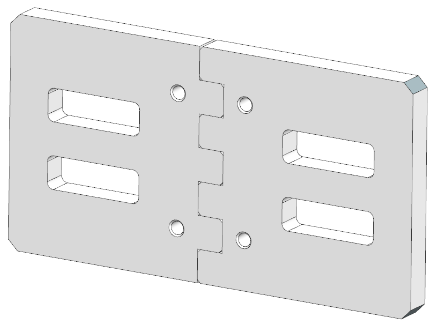
\includegraphics[width=\textwidth]{04_Anwendung_und_Aufbau/Montageschritt_1}
			\caption{Montageschritt 1}
			\label{fig:Montageschritt 1}
		\end{subfigure}
		\hfill
		\begin{subfigure}[b]{0.3\textwidth}
			\centering
			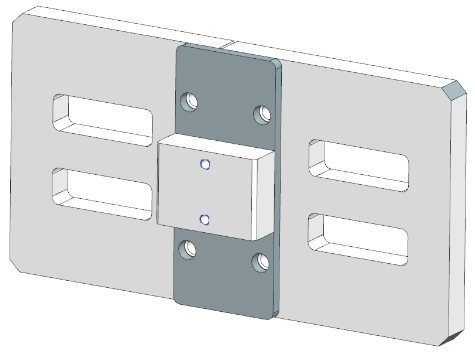
\includegraphics[width=\textwidth]{04_Anwendung_und_Aufbau/Montageschritt_2}
			\caption{Montageschritt 2}
			\label{fig:Montageschritt 2}
		\end{subfigure}
		\hfill
		\begin{subfigure}[b]{0.3\textwidth}
			\centering
			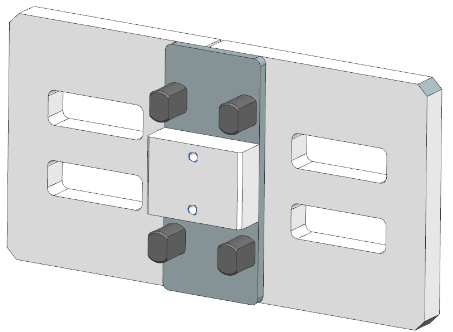
\includegraphics[width=\textwidth]{04_Anwendung_und_Aufbau/Montageschritt_3}
			\caption{Montageschritt 3}
			\label{fig:Montageschritt 3}
		\end{subfigure}
		\caption{Anwendungsteilprozesse}
		\label{fig:Montageschritte}
	\end{figure}
	
	\begin{bfhNoteBox}
		Alle Detailzeichnungen in Fertigungsdaten werden im Anhang beigelt. 
	\end{bfhNoteBox}	
	
	\vspace{5mm} 
	\begin{wrapfigure}{r}{0.6\textwidth}
		\centering
		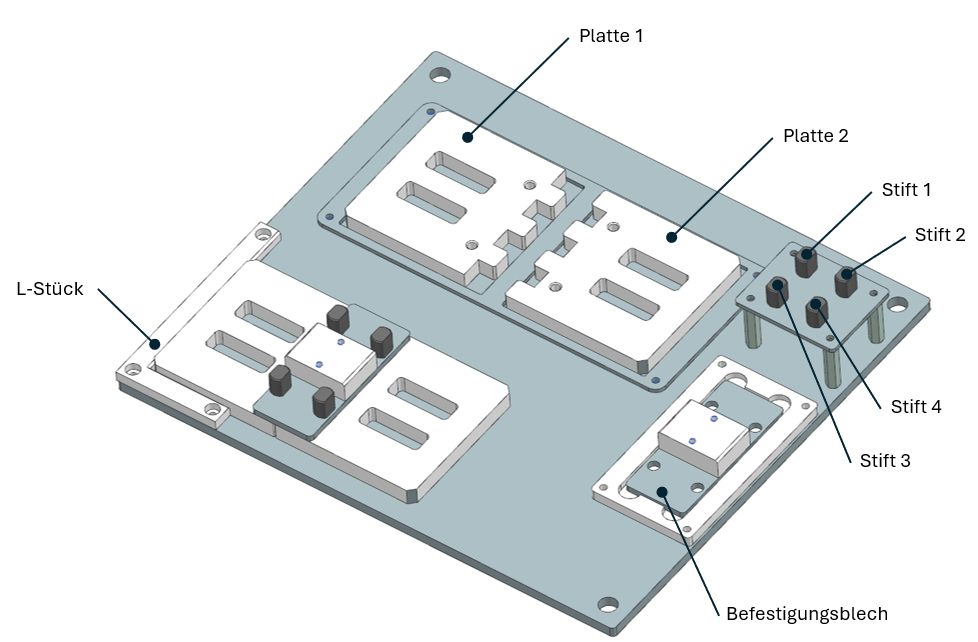
\includegraphics[width=0.6\textwidth]{04_Anwendung_und_Aufbau/Montagevorrichtung}
		\captionsetup{justification=centering}
		\caption{Montagevorrichtung}
		\label{fig:Montagevorrichtung}
	\end{wrapfigure} \par
	Die Montage wird auf einer Platte durchgeführt, welche gleichzeitig auch als Halterung für Komponenten dient (\ref{fig:Montagevorrichtung}). Im unteren linken Bereich werden die Komponenten montiert. Dafür wird das Kunststoff-L-Stück als Anschlag verwendet. 
	
	